\documentclass[10pt]{article}
\usepackage[slovene]{babel}
\usepackage[utf8]{inputenc}
\usepackage[T2A]{fontenc}
\usepackage{amsmath}
\usepackage{amsfonts}
\usepackage{amssymb}
\usepackage[version=4]{mhchem}
\usepackage{stmaryrd}
\usepackage{graphicx}
\usepackage[export]{adjustbox}
\graphicspath{ {./images/} }
\usepackage{physics}
\usepackage{geometry}
\geometry{left=2cm,right=2cm,top=2cm,bottom=2cm}



\title{Frank-Hertzov poskus}
\author{Samo Krejan}
\date{marec 2025}


\begin{document}
\maketitle

\section{Uvod}

Frank-Hertzov poskus je zgodovinsko izredno pomemben za kvantno mehaniko saj je leta 1914 kot prvi potrdil diskretizacijo stanj atoma.

Plinska trioda vsebuje kaplico živega srebra $Hg$, ki ima nad sabo pri temperaturi $200^{\circ}C$ tlak približno $1 \ kPa$. V cevi pospešujemo elektrone z napetostjo $U_1$ od katode proti anodni mrežici in jih nato lovimo s kolektorsko anodo, ki elektrone odbija z majhno napetostjo $U_2$. Namen tega je zmanševanje motenj ozadja. Kar merimo je tok elektronov $I_2$, ki uspe premagati potencial $U_2$ in doseči kolektorsko anodo.

Med katodo in anodno mrežico se atomi pospešujejo, hkrati pa se trkajo v atome $Hg$. Trki so elastični ko je energija elektronov manjša od $\Delta E = E_1 - E_0$, kjer sta $E_0$ in $E_1$ osnovno in prvo vzbujeno stanje elektrona v zunanji lupini atoma $Hg$. Pri večjih energijah je možnost za neelastičen trk dovolj velika, tako da so v vmesnem prostoru med katodo in anodno mrežico l elektroni z energijo manjšo od $\Delta E$. To sicer velja le ob dovolj veliki gostoti atomov, tako da elektroni ne morejo dobiti več energije pred trkom. Pri manjši gostoti (nižji temperaturi) ali pri višji pospeševalni napetosti dobijo elektroni več energije in lahko atome vzbudijo tudi v druga vzburjena stanja ali jih celo ionizirajo - dobimo plazmo, ki jo lahko opazimo kot svetlobo v celici. Plazma ustvari popolnoma drugačne pogoje s katerimi se v tej vaji ne ukvarjamo.

Ko spreminjamo napetost $U_1$ se spreminja povprečna kinetična energija elektronov, dokler ne dosežemo napetosti $U_1 = \Delta E / e_0$, kjer je $e_0$ osnovni naboj - naboj elektrona. Takrat pride do neelastičnih trkov in kinetična energija elektronov pade na $0$. Če to napetost še naprej večamo se elektroni, ki so se umes ustavili, spet pospešijo in če pridejo spet do energije $\Delta E$ lahko vzbudijo še en atom iz osnovnega stanja. To se seveda ponavlja, če še naprej večamo napetost.

Nas zanimajo predvsem elektroni blizu anodnege mrežice - te elektrone polovimo z anodnim kolektorjem če le imajo dovolj kinetične energije za premostitev potenciala $U_2$ in so pravilno usmerjeni.

Shema eksperimenta je prikazana na sliki \ref{shema}

\begin{figure}[h]
\begin{center}
    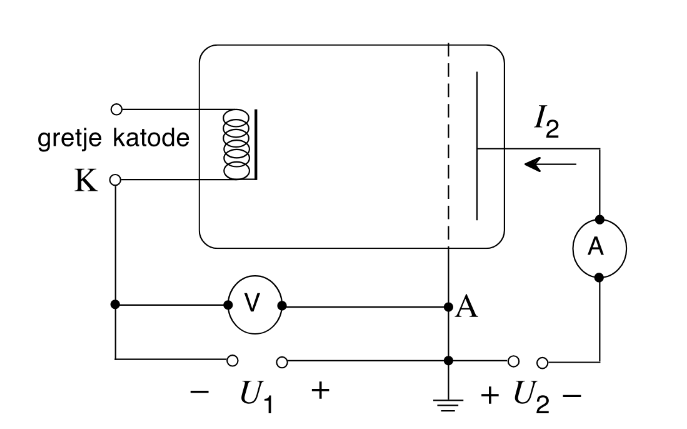
\includegraphics[width=10 cm]{shema.png}
    \caption{Shema Franck-Hertzovega poskusa. Vir: navodila}
    \label{shema}
\end{center}
\end{figure}

\section{Potrebščine}

\begin{itemize}
    \item Frank - Hertzova cev v termostiranem ohišju,
    \item kontrolna enota za ustvarjanje žagaste napetosti ($U_1$), izvor izmenične napetosti za gretje katode ($U_H$), merjenje temperature,
    \item digitalni osciloskop (Siglent SDS2202X-E),
    \item USB ključek za shranjevanje podatkov.
\end{itemize}

\section{Naloga}

\begin{enumerate}
    \item Opazuj odvisnost toka $I_2$ med anodno mrežico in anodnim kolektorjem v odvisnosti od negativne napetost $U_1$ na katodi. Spreminjaj temperaturo in posebej natančno opazuj in izmeri položaje vseh vrhov v merjenih odvisnostih. Skiciraj odvisnosti pri petih različnih temperaturah, ko se slike primerno razlikujejo, to je približno pri temperaturah okoli $180$, $160$, $140$ in $120^{\circ}C$.
    \item Natančno določi položaje vrhov $U_{1,n} = U_2 + n\Delta E/e_0$ pri posameznih temperaturah in rezultate vnesi v tabelo. Razlike napetosti med zaporednimi maksimumi ustrezajo energiji, ki jo izgubijo elektroni pri posameznem neelastičnem trku z atomom $Hg$. Določi $\Delta E = E_1 - E_0 = e_0 \Delta U_1$, kjer sta $E_1$ in $E_0$ energiji prvega vzbujenega in osnovnega stanja elektrona v zunanji lupini $Hg$.
\end{enumerate}

\section{Rezultati in analiza}

Eksperiment smo izvajali pri petih različnih temperaturah: $180^{\circ}C, 160^{\circ}C, 140^{\circ}C, 120^{\circ}C$, kjer smo uporabili nastavitve predlagane v navodilih (glej \ref{nastavitve}), ter pri $40^{\circ}C$, kjer je bila $U_1$ nastavljena na $18V$, saj sem imel drugače probleme s plazmo. Rezultate eksperimentov lahko prikažemo na grafih, najprej pri vsaki temperaturi posebaj potem pa še vse na istem grafu (\ref{posebej}, \ref{vsi})

\begin{figure}[h]
    \begin{center}
        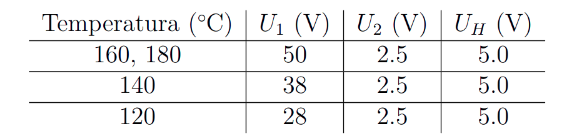
\includegraphics[width=10cm]{nastavitve.png}
        \caption{Priporočene nastavitve za posamezne temperature. Vir: navodila}
        \label{nastavitve}
    \end{center}
\end{figure}

Iz grafov se že takoj lepo vidi, da so vrhovi razmaknjeni enakomerno, kar potrjuje teorijo (to bomo pokazali še malo kasneje), predvsem pa se vidi tudi da lokacije vrhov niso odvisne od temperature - spremeni se le tok, saj se pri nižji temperaturi (nižji gostoti $Hg$ plina) očitno poveča prepustnost elektronov.
\newpage
\begin{figure}[h]
    \begin{center}
        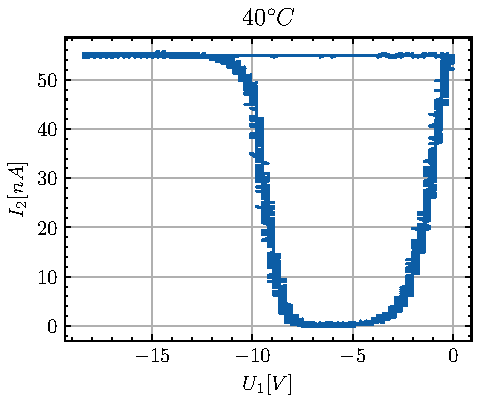
\includegraphics[width=5cm]{40.pdf}
        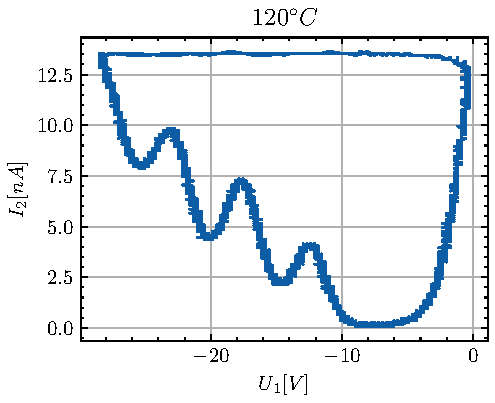
\includegraphics[width=5cm]{120.pdf}
        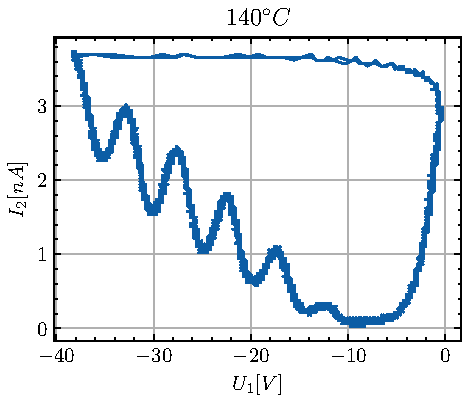
\includegraphics[width=5cm]{140.pdf}
        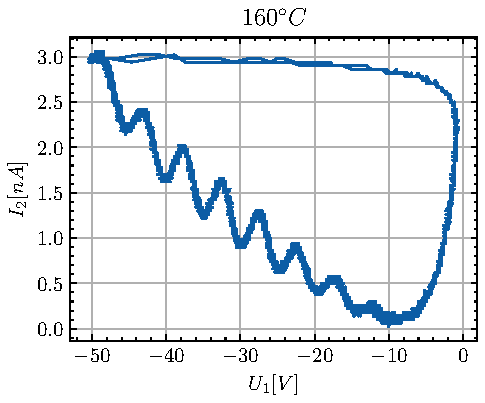
\includegraphics[width=5cm]{160.pdf}
        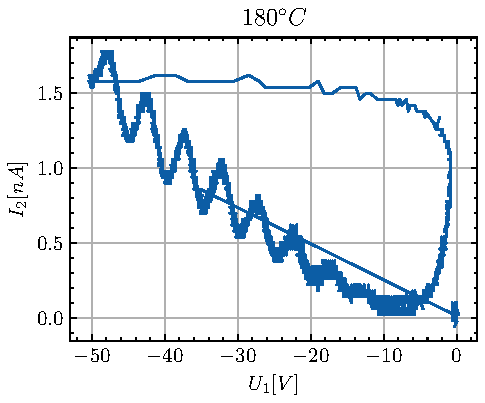
\includegraphics[width=5cm]{180.pdf}
        \caption{Meritev pri vsaki temperaturi posebaj}
        \label{posebej}
    \end{center}
\end{figure}

\begin{figure}[h]
    \begin{center}
        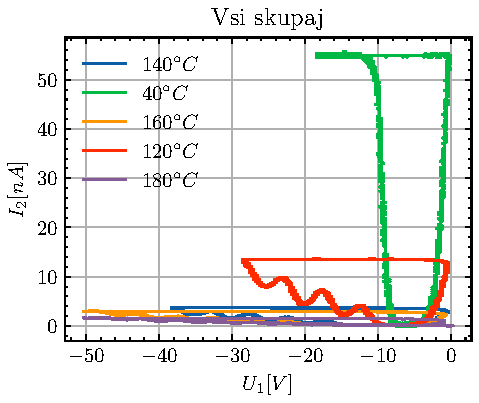
\includegraphics[width=8cm]{vsi.pdf}
        \caption{Vse meritve na istem grafu}
        \label{vsi}
    \end{center}
\end{figure}


Kar nam preostane storiti, je iz grafov kjer se to da (ne pri $40$ stopinjah) odčitati $\Delta E$, skupaj z napako, ki jo lahko ocenimo iz širine vrhov. Najprej bomo vse pozicije vrhov predstavili v tabeli \ref{vrhovi}. Bralec naj je pozoren da smo navedli absolutne vrednosti napetosti. Napako napetosti vrhov ocenimo na $0,4\ V$ na podlagi oblike in širine vrhov.

\newpage

\begin{table}[ht]
    \begin{center}
    \begin{tabular}{l|lllllll}
    T\textbackslash{}U & 1    & 2    & 3    & 4    & 5    & 6    & 7    \\ \hline
    120                & 12,5 & 17,6 & 22,9 & /    & /    & /    & /    \\
    140                & 12,3 & 17,4 & 22,5 & 27,7 & 32,9 & /    & /    \\
    160                & /    & 17,4 & 22,5 & 27,6 & 32,6 & 37,7 & 43,3 \\
    180                & /    & /    & 22,5 & 27,5 & 32,4 & 37,5 & 42,8
    \end{tabular}
    \caption{Napetost pri kateri se pojavijo vrhovi v voltih v odvisnosti od temperature v stopinjah celzija}
    \label{vrhovi}
    \end{center}
\end{table}



Sedaj lahko določimo $\Delta E$ pri vsaki temperaturi posebaj in nato še povprečje pri vseh temperaturah. Z upoštevanjem napak to naredimo na sledeč način:

\begin{enumerate}
    \item izračunamo razlike sosednjih vrednosti v tabeli. Statistika nas nauči, da imajo te razlike napako $\sqrt{2} \cdot 0,4$ kjer je $0,4$ napaka posamezne meritve,
    \item pri vsaki temperaturi in nato še za vse skupaj izračunamo povprečje teh razlik. Napaka je tu izračunana kot $\sqrt{\frac{2}{N}}\cdot 0,4$, kjer je $N$ število razlik ki smo jih upoštevali,
    \item glede na majhno količino podatkov lahko napaki prištejemo (pitagorejsko) kar tudi največji odmik podatkov od povprečja, oziroma, ko računamo povprečje čez vse temperature, lahko za to napako upoštevamo samo 2/3 razlik, saj je teh dovolj.
\end{enumerate}

To nas privede do tabele s poslednjimi rezultati \ref{rezultati}:

\begin{table}[h]
    \begin{center}
    \begin{tabular}{l|l|l}
    T [$^{\circ}C$]  & $\Delta E$  [$eV$] & $\sigma_E$ [$eV$] \\ \hline
    120 & 5,2 & 0,5   \\
    140 & 5,2 & 0,3   \\
    160 & 5,2 & 0,7   \\
    180 & 5,1 & 0,5   \\
    vsi & 5,1 & 0,2  
    \end{tabular}
    \caption{Tabela rezultatov eksperimenta}
    \label{rezultati}
    \end{center}
\end{table}


Prva stvar, ki jo opazimo je, da res velja da je $\Delta E$ neodvisen od temperature. Namreč rezultati se v okviru napake med sabo strinjajo. Poleg tega se rezultati skladajo tudi s teorijo. Literatura namreč navaja vrednost $\Delta E = 4,9\ eV$. Torej smo lahko precej zadovoljni za našim eksperimentom.

\end{document}